\begin{enumerate}[label=\thechapter.\arabic*,ref=\thechapter.\theenumi]

\item Discrete signals $x\brak{n}$ and $y\brak{n}$ are shown below. The cross-correlation $r_{xy}\brak{0}$ is:
\begin{figure}[H]
    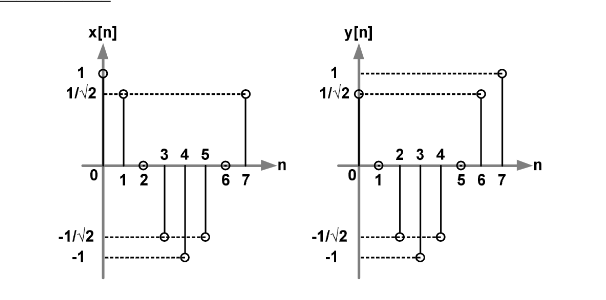
\includegraphics[width=1\columnwidth]{2022/BM/15/figs/question_BM_15.png}
    \caption{Question Figure}
    \label{fig:question_fig}
\end{figure}\hfill{(GATE BM 2022)}\\
\solution
\iffalse
\let\negmedspace\undefined
\let\negthickspace\undefined
\documentclass[journal,12pt,twocolumn]{IEEEtran}
\usepackage{cite}
\usepackage{amsmath,amssymb,amsfonts,amsthm}
\usepackage{algorithmic}
\usepackage{graphicx}
\usepackage{textcomp}
\usepackage{xcolor}
\usepackage{txfonts}
\usepackage{listings}
\usepackage{enumitem}
\usepackage{mathtools}
\usepackage{float}
\usepackage{gensymb}
\usepackage{comment}
\usepackage[breaklinks=true]{hyperref}
\usepackage{tkz-euclide} 
\usepackage{listings}
\usepackage{gvv}                                        
\def\inputGnumericTable{}                                 
\usepackage[latin1]{inputenc}                                
\usepackage{color}                                            
\usepackage{array}          
\usetikzlibrary{positioning, arrows.meta}
\usepackage{longtable}                                       
\usepackage{calc}                                             
\usepackage{multirow}                                         
\usepackage{hhline}                                           
\usepackage{ifthen}                                           
\usepackage{lscape}
\usepackage{amsmath}
\newtheorem{theorem}{Theorem}[section]
\newtheorem{problem}{Problem}
\newtheorem{proposition}{Proposition}[section]
\newtheorem{lemma}{Lemma}[section]
\newtheorem{corollary}[theorem]{Corollary}
\newtheorem{example}{Example}[section]
\newtheorem{definition}[problem]{Definition}
\newcommand{\BEQA}{\begin{eqnarray}}
\newcommand{\EEQA}{\end{eqnarray}}
\newcommand{\define}{\stackrel{\triangle}{=}}
\theoremstyle{remark}
\newtheorem{rem}{Remark}
\begin{document}

\bibliographystyle{IEEEtran}
\title{GATE-BM-Q15}
\author{EE23BTECH11015 - DHANUSH V NAYAK$^{*}$% <-this % stops a space
}
\maketitle
\newpage
\bigskip
\renewcommand{\thefigure}{\arabic{figure}}
\renewcommand{\thetable}{\theenumi}
\textbf{Question:} Discrete signals $x\brak{n}$ and $y\brak{n}$ are shown below. The cross-correlation $r_{xy}\brak{0}$ is:
\begin{figure}[H]
    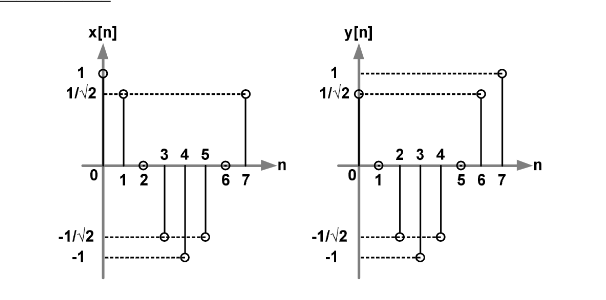
\includegraphics[width=1\columnwidth]{2022/BM/15/figs/question_BM_15.png}
    \caption{Question Figure}
    \label{fig:question_fig}
\end{figure}\hfill{(GATE BM 2022)}\\
\solution
\fi
\begin{table}[H]
\centering
\renewcommand\thetable{1}
\setlength{\extrarowheight}{9pt}
\resizebox{0.5\textwidth}{!}{
\begin{tabular}{|c|c|c|}
\hline
\textbf{Parameter} & \textbf{Description} & \textbf{Value} \\ \hline
$x\brak{n}$ & First Sequence & $x(n) = 
\begin{cases}
    0 & ; n < 0 \\
    \brak{1,\frac{1}{\sqrt{2}} , 0 ,-\frac{1}{\sqrt{2}},-1,-\frac{1}{\sqrt{2}},0,\frac{1}{\sqrt{2}}} & ; 0 \leq n \leq 7 \\
    0 & ; n > 7 \\
\end{cases}$   \\ \hline
$y\brak{n}$ &Second Sequence &$y(n) = 
\begin{cases}
    0 & ; n < 0 \\
    \brak{\frac{1}{\sqrt{2}} , 0 ,-\frac{1}{\sqrt{2}},-1,-\frac{1}{\sqrt{2}},0,\frac{1}{\sqrt{2}},1} & ; 0 \leq n \leq 7 \\
    0 & ; n > 7 \\
\end{cases}$  \\ \hline
$r_{xy}\brak{k}$& Cross-correlation & $\sum_{m=-\infty}^{\infty} x\brak{m}y\brak{m-k}$ \\ \hline 
\end{tabular}}
\caption{Parameter Table}
\label{tab:gate_bm_Q15}
\end{table}

It can be seen that :
\begin{align}
    y\brak{n} = x\brak{n+1}\label{eq:gate_bm_q15.1}
\end{align}
From \tabref{tab:gate_bm_Q15} :
\begin{align}
    r_{xy}\brak{k} &= \sum_{m=-\infty}^{\infty} x\brak{m}y\brak{m-k}\\
                &= x\brak{k} * y\brak{-k}
\end{align}
From \eqref{eq:gate_bm_q15.1}:
\begin{align}
    r_{xy}\brak{k} &= x\brak{k+1} * x\brak{-k}\\
                &= \sum_{n=-\infty}^{\infty} x\brak{n+1}x\brak{n+k} 
\end{align}
By definition of x\brak{n} from \tabref{tab:gate_bm_Q15}:
\begin{align}
     r_{xy}\brak{k} &= \sum_{n=0}^{6} x\brak{n+1}x\brak{n+k} \\
     r_{xy}\brak{0} &= \sum_{n=0}^{6} x\brak{n+1}x\brak{n} 
\end{align}
Using values from \figref{fig:question_fig}:
\begin{align}
    r_{xy}\brak{0} &= 2\sqrt{2}
\end{align}
\begin{figure}[H]
    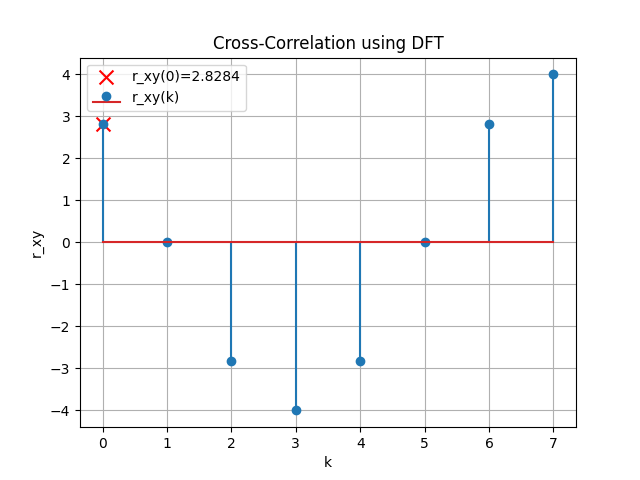
\includegraphics[width=1\columnwidth]{2022/BM/15/figs/cross-corelation.png}
    \caption{Verification of result by DFT}
    \label{fig:cross-corelation}
\end{figure}

%\end{document}


\pagebreak


\item 
Which one of the following is the closed form for the generating function of the sequence $ \bigl\{ a \bigl\}_{n \geq0}$ defined below?
\begin{equation}
a_n=
    \begin{cases}
        n+1 & , \text{n is odd}\\
        1 & \text{otherwise}
    \end{cases}
\end{equation}\label{eq: 22cs361}


\begin{enumerate}
    \item[(A)] $ \frac{x\brak{1+x}^2}{\brak{1-x^2}^2} + \frac{1}{1-x}$
    \item[(B)]$ \frac{x\brak{3-x^2}}{\brak{1-x^2}^2} + \frac{1}{1-x}$
    \item[(C)] $ \frac{2x}{\brak{1-x^2}^2} + \frac{1}{1-x}$
    \item[(D)] $ \frac{x}{\brak{1-x^2}^2} + \frac{1}{1-x}$  
\end{enumerate}
\hfill(GATE CS 2022 QUESTION 36)\\
\solution
 \iffalse
\let\negmedspace\undefined
\let\negthickspace\undefined
\documentclass[journal,12pt,twocolumn]{IEEEtran}
\usepackage{cite}
\usepackage{amsmath,amssymb,amsfonts,amsthm}
\usepackage{algorithmic}
\usepackage{graphicx}
\usepackage{textcomp}
\usepackage{xcolor}
\usepackage{txfonts}
\usepackage{listings}
\usepackage{enumitem}
\usepackage{mathtools}
\usepackage{gensymb}
\usepackage{comment}
\usepackage[breaklinks=true]{hyperref}
\usepackage{tkz-euclide}
\usepackage{listings}
\usepackage{gvv}
\def\inputGnumericTable{}
\usepackage[latin1]{inputenc}
\usepackage{color}
\usepackage{array}
\usepackage{longtable}
\usepackage{calc}
\usepackage{multirow}
\usepackage{hhline}
\usepackage{ifthen}
\usepackage{lscape}

\newtheorem{theorem}{Theorem}[section]
\newtheorem{problem}{Problem}
\newtheorem{proposition}{Proposition}[section]
\newtheorem{lemma}{Lemma}[section]
\newtheorem{corollary}[theorem]{Corollary}
\newtheorem{example}{Example}[section]
\newtheorem{definition}[problem]{Definition}
\newcommand{\BEQA}{\begin{eqnarray}}
\newcommand{\EEQA}{\end{eqnarray}}
\newcommand{\define}{\stackrel{\triangle}{=}}
\theoremstyle{remark}
\newtheorem{rem}{Remark}
\begin{document}

\bibliographystyle{IEEEtran}
\vspace{3cm}

\title{GATE 2022  -AE 63}
\author{EE23BTECH11057 - Shakunaveti Sai Sri Ram Varun$^{}$% &lt;-this % stops a space
}
\maketitle
\newpage
\bigskip
\vspace{2cm}
\textbf{Question: }
Which one of the following is the closed form for the generating function of the sequence $ \bigl\{ a \bigl\}_{n \geq0}$ defined below?
\begin{equation}
a_n=
    \begin{cases}
        n+1 & , \text{n is odd}\\
        1 & \text{otherwise}
    \end{cases}
\end{equation}\label{eq: 22cs361}


\begin{enumerate}
    \item[(A)] $ \frac{x\brak{1+x}^2}{\brak{1-x^2}^2} + \frac{1}{1-x}$
    \item[(B)]$ \frac{x\brak{3-x^2}}{\brak{1-x^2}^2} + \frac{1}{1-x}$
    \item[(C)] $ \frac{2x}{\brak{1-x^2}^2} + \frac{1}{1-x}$
    \item[(D)] $ \frac{x}{\brak{1-x^2}^2} + \frac{1}{1-x}$  
\end{enumerate}
\hfill(GATE CS 2022 QUESTION 36)\\
\textbf{Solution}:\\
\fi
\begin{table}[h!] 
\centering
\begin{tabular}{|c|c|c|}
   \hline
    \textbf{Parameter} & \textbf{Description} & \textbf{Value} \\
   \hline
   $ X\brak{z}$ & Generating function for a sequence $\bigl\{ a_n \bigl\}$ & ? \\
   \hline
   \multirow{2}{*}{$a_n$} & $n^{th}$ term of the sequence & $\brak{n+1}u\brak{n}$ (when odd) \\
   \cline{3-3}
   & & $u\brak{n}$ (when even) \\
   \hline
\end{tabular}

\caption{input values}
\label{tab: Table2022cs36}
\end{table}
For the given sequence:
\begin{align}
X\brak{z} &= \sum_{k=-\infty}^{\infty} u\brak{2k} z^{-2k}+ \sum_{k=-\infty}^{\infty} \brak{\brak{2k+2}u\brak{2k+1}} z^{-\brak{2k+1}}\\
\implies X\brak{z} &= \brak{1+z^{-2}+z^{-4} + \dots} + \brak{2z^{-1}+4z^{-3} + 6z^{-5} + \dots}\\
\implies X\brak{z} &= \frac{1}{1-z^{-2}} + \brak{2z^{-1}+4z^{-3}+6z^{-5} \dots} \quad |z|>1\\
\implies X\brak{z} &= \frac{1}{1-z^{-2}} +2z^{-1}\brak{\frac{1}{1-z^{-2}}+\frac{z^{-2}}{\brak{1-z^{-2}}^2}} \quad |z|>1
\end{align}
\begin{align}
\therefore X\brak{z} &= \frac{1}{1-z^{-1}} + \frac{z^{-1}\brak{1+z^{-2}}}{\brak{1-z^{-2}}^2} \quad |z|>1 \label{eq: 22cs36_1}
\end{align}
\eqref{eq: 22cs36_1} is the closed form of generating function required in the question.\\
Hence, option (A) is correct.\\\\
\begin{align}
X\brak{z}&=X_1\brak{z}+X_2\brak{z}\\
X_1\brak{z}&=\frac{1}{1-z^{-1}} \quad |z|>1\\ 
\implies x_1\brak{n} &= u\brak{n}\\
\implies a_n&=  x_1\brak{n}+ x_2\brak{n}
\end{align}
To find inverse z-transform of $ X_2\brak{z}$ we use contour integration technique:
\begin{align}
    x_2\brak{n}&=\frac{1}{2\pi j}\oint_{C}X_2\brak{z} \;z^{n-1} \;dz  \\
    &=\frac{1}{2\pi j}\oint_{C}\frac{z^{n}\brak{z^2+1}}{\brak{z^2-1}^2} \;dz 
\end{align}

We can observe that we have two poles at \\$ z= 1,-1$. And poles are repeated twice, thus by applying residue theorem two times for poles 1 and -1:
\begin{align}
    x_2\brak{n}&=\frac{1}{\brak {1}!}\lim\limits_{z\to 1}\frac{d}{dz}\brak {{(z-1)}^{2}X_2\brak{z}} + \frac{1}{\brak {1}!}\lim\limits_{z\to -1}\frac{d}{dz}\brak {{(z+1)}^{2}X_2\brak{z}} \\
\implies    x_2\brak{n} &=\lim\limits_{z\to 1}\frac{d}{dz}\brak {{(z-1)}^{2}\frac{z^n\brak{z^2+1}}{{(z^2-1)}^2}}+ \lim\limits_{z\to -1}\frac{d}{dz}\brak {{(z+1)}^{2}\frac{z^n\brak{z^2+1}}{{(z^2-1)}^2}}   \\
\notag \implies x_2\brak{n} &= \lim\limits_{z\to 1}\frac{\brak{z+1}^2\brak{nz^{n-1}+ \brak{n+2}z^{n+1}}-2z^n\brak{1+z^2}\brak{z+1}}{\brak{z+1}^4}\\
    &+ \lim\limits_{z\to -1}\frac{\brak{z-1}^2\brak{nz^{n-1}+ \brak{n+2}z^{n+1}}-2z^n\brak{1+z^2}\brak{z-1}}{\brak{z-1}^4}
\end{align}
on simplification, we get
\begin{align}
x_2\brak{n} &= \frac{n+n\brak{-1}^{n-1}}{2}\\
\therefore a_n &= u\brak{n} + \frac{n+n\brak{-1}^{n-1}}{2} u\brak{n}
\end{align}
Which is the sequence given in the Question.

\begin{figure}[h!]
    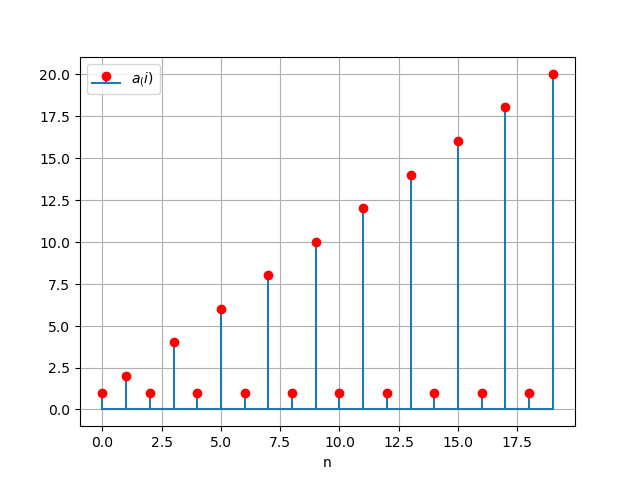
\includegraphics[width = \columnwidth]{2022/CS/36/figs/Figure_1.png}
    \caption{Terms of the sequence given}
    \centering
    \label{fig: nm_63_fig_2}
\end{figure}



\newpage
\item
\textbf{Question:}
Consider the following recurrence:
\begin{align}
	f(1)\;\;&=\;\;1;\label{g2-1cs.51}\\
	 f(2n)\;\;&=\;2f(n)-1,\text{  for $n\geq$1;}\label{g2-2cs.51}\\
	 f(2n+1)\;\;&=\;2f(n)+1,\text{  for $n\geq$1.}\label{g2-3cs.51}
\end{align}
Then, which of thefollowing is/are \textbf{TRUE?}\\
(A) $f(2^n-1)\;=\;2^n-1$\\
(B) $f(2^n)\;=\;1$\\
(C) $f(5\cdot2^n)\;=\;2^{n+1}+1$\\
(D) $f(2^n+1)\;=\;2^n+1$\\
\hfill{[GATE-CS.51 2022]}\\
\solution
 \iffalse
\let\negmedspace\undefined
\let\negthickspace\undefined
\documentclass[journal,12pt,twocolumn]{IEEEtran}
\usepackage{xparse}
\usepackage{cite}
\usepackage{amsmath,amssymb,amsfonts,amsthm}
\usepackage{algorithmic}
\usepackage{graphicx}
\usepackage{textcomp}
\usepackage{xcolor}
\usepackage{txfonts}
\usepackage{listings}
\usepackage{enumitem}
\usepackage{mathtools}
\usepackage{gensymb}
\usepackage{comment}
\usepackage[breaklinks=true]{hyperref}
\usepackage{tkz-euclide} 
\usepackage{listings}
\usepackage{gvv}                                        
\def\inputGnumericTable{}                                 
\usepackage[latin1]{inputenc}                                
\usepackage{color}                                            
\usepackage{array}                                            
\usepackage{longtable}                                       
\usepackage{calc}                                             
\usepackage{multirow}                                         
\usepackage{hhline}                                           
\usepackage{ifthen}                                           
\usepackage{lscape}

\newtheorem{theorem}{Theorem}[section]
\newtheorem{problem}{Problem}
\newtheorem{proposition}{Proposition}[section]
\newtheorem{lemma}{Lemma}[section]
\newtheorem{corollary}[theorem]{Corollary}
\newtheorem{example}{Example}[section]
\newtheorem{definition}[problem]{Definition}
\newcommand{\BEQA}{\begin{eqnarray}}
\newcommand{\EEQA}{\end{eqnarray}}
\newcommand{\define}{\stackrel{\triangle}{=}}
\theoremstyle{remark}
\newtheorem{rem}{Remark}
\begin{document}

\bibliographystyle{IEEEtran}
\vspace{3cm}

\title{GATE-CS.51}
\author{EE23BTECH11046 - Poluri Hemanth$^{*}$}
\maketitle
\textbf{Question:}
Consider the following recurrence:
\begin{align}
	f(1)\;\;&=\;\;1;\label{g2-1cs.51}\\
	 f(2n)\;\;&=\;2f(n)-1,\text{  for $n\geq$1;}\label{g2-2cs.51}\\
	 f(2n+1)\;\;&=\;2f(n)+1,\text{  for $n\geq$1.}\label{g2-3cs.51}
\end{align}
Then, which of thefollowing is/are \textbf{TRUE?}\\
(A) $f(2^n-1)\;=\;2^n-1$\\
(B) $f(2^n)\;=\;1$\\
(C) $f(5\cdot2^n)\;=\;2^{n+1}+1$\\
(D) $f(2^n+1)\;=\;2^n+1$\\
\hfill{[GATE-CS.51 2022]}\\
\textbf{Solution:}\\
\fi
(A)\\
let $x(2^k-1)=2^k-1$ for any $k\geq1$,
\begin{align}
	x(2^{k+1}-1)&=x(2(2^k-1)+1)
\end{align}
From \eqref{g2-3cs.51},
\begin{align}
	&=2x(2^k-1)+1\\
        &=2(2^k-1)+1\\
	&=2^{k+1}-1\label{1.cs51}
\end{align}
From \eqref{g2-1cs.51},\eqref{1.cs51}
\begin{align}
	x(2-1)&=2-1\text{  ($k=0$)}\\
	&=1
\end{align}
Hence $x(2^n-1)=2^n-1$ for $n\geq1$\\
So statement A is TRUE\\
\\(B)\\
Let $x(2^k)=1$ for any $k\geq$0
\begin{align}
	x(2^{k+1})&=x(2\cdot2^k)
\end{align}
From \eqref{g2-2cs.51}
\begin{align}
	&=2x(2^k)-1\label{2cs.51}\\
	&=1
\end{align}
From \eqref{2cs.51},\eqref{g2-2cs.51}
\begin{align}
	x(2)&=2x(1)-1\\
	&=1\label{bcs.51}
\end{align}
Hence $x(2^n)=1$ for every $n\geq0$ value.\\
So statement B is TRUE.\\
\\(C)\\
Let,$x(5\cdot2^k)=2^{k+1}+1$ be true for any $k\geq0$,
\begin{align}
	x(5\cdot2^{k+1})&=x(2(5\cdot2^k))
\end{align}
From \eqref{g2-2cs.51}
\begin{align}
	&=2x(5\cdot2^k)-1\\
	&=2^{k+2}+1\label{3cs.51}
\end{align}
$k=-1$ ,From \eqref{3cs.51}
\begin{align}
	x(5)&=2^1+1\\
	&=3
\end{align}
Proof:-
\begin{align}
        x(5)&=x(2\cdot2+1)
\end{align}
From \eqref{g2-3cs.51},\eqref{bcs.51}
\begin{align}
        &=2x(2)+1\\
        &=3
\end{align}
Hence $x(5.2^n)=2^{n+1}+1$ for $n\geq1$\\
So statement C is TRUE.\\
\\(D)
\begin{align}
	x(2^n+1)&=x(2\cdot2^{n-1}+1)
\end{align}
From \eqref{g2-3cs.51},\eqref{bcs.51}
\begin{align}
	&=2x(2^{n-1})+1\\
	&=3
\end{align}
Hence statement D is FALSE.
\begin{figure}
	\centering
	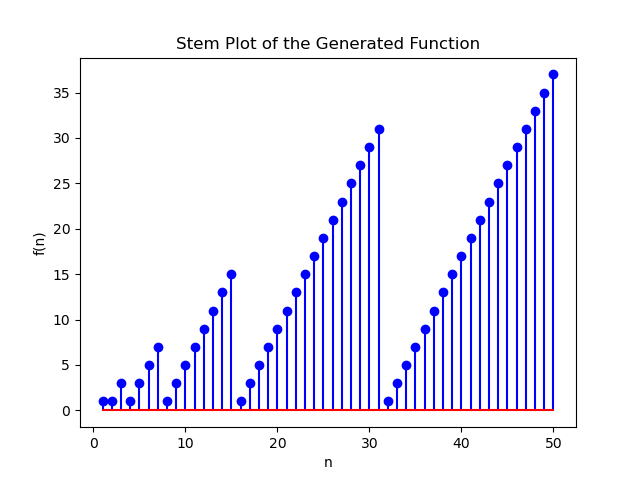
\includegraphics[width=1\columnwidth]{2022/CS/51/figures/gate2.png}
	\caption{plot of $x(n)$}
	\label{cs.51.stem}
\end{figure}







%\end{document}

\end{enumerate}

